\part{SW 04 - Data Link Layer - Sicherungsschicht}\label{part:sw04}
\section{Lernziele (Leitfragen)}
\begin{itemize}
    \item Was ist der Unterschied zwischen CSMA/CD und CSMA/CA? Wo werden sie verwendet?
    \item Was ist der Zweck der Sicherungsschicht?
    \item Wie ist die Sicherungsschicht aufgeteilt? Was ist die Hauptaufgabe der LLC und MAC Schichten?
    \item Welches sind die am häufigsten verwendeten Zugriffsverfahren?
    \item Was für Felder findet man in der Sicherungsschicht Frame?
    \item Was sind die wichtigsten Merkmale von MAC Adressen?
    \item Was machen Endgeräte, wenn ihre NIC ein Frame im Medium erkennen?
    \item Wie werden Sicherungsschicht Frames in einem Switch bearbeitet?
    \item Wie funktioniert der «Learn-and-forward» Prozess?
    \item Was ist der Unterschied zwischen «Unicast» und «Broadcast» Frames?
    \item Was ist der Zweck ARPs?
    \item Wie funktioniert ARP?
\end{itemize}

\section{Antworten}
\subsection*{Was ist der Unterschied zwischen CSMA/CD und CSMA/CA? Wo werden sie verwendet?}\label{sub:csma}\index{CSMA - Carrier Sense Multiple Access}
//TODO Sollte für die Logik zu SW03 T1 verschoben werden.\\

\textbf{CSMA: Carrier Sense Multiple Access}
\begin{itemize}
    \item Sender hört den Datenverkehr auf der Leitung ab (= carrier sense)
    \item Sender wartet, bis der Kanal frei ist
    \item sobald der Kanal frei ist, darf gesendet werden
    \item falls mehrere Sender (fast) gleichzeitig anfangen zu senden:\\Kollision $\rightarrow$ Wiederholung nach zufälliger Zeitspanne
\end{itemize}\,\\

\textbf{CSMA/CA (CA = Collision Avoidance)}
\begin{itemize}
    \item Kollisionsvermeidung durch zufällige Wartezeit nach Erkennung eines freien Kanals
    \item z.B. WLAN 802.11-DCF (Distributed Coordination Function)
\end{itemize}\,\\

\textbf{CSMA/CD (Collision Detection)}
\begin{itemize}
    \item sobald eine Kollision erkannt wird, wird die Übertragung abgebrochen
    \item z.B. Ethernet
\end{itemize}\,\\

\begin{tabularx}{\textwidth}{X|X}
    \multicolumn{1}{X}{CSMA/CD}&\multicolumn{1}{X}{CSMA/CA}\\
    \hline
    $\bullet$ Greift nach der Kollision&$\bullet$ Greift vor der Kollision\\
    $\bullet$ Genutzt in kabelgebundenen Netzwerken&$\bullet$ Genutzt in kabellosen Netzwerken\\
    $\bullet$ Reduziert die `'recovery time'' nach einer Kollision&$\bullet$ Minimiert Kollisionsgefahr\\
    $\bullet$ Bei Konflikt wird erneut gesendet&$\bullet$ Sendet zuerst die Info, dass etwas übermittelt wird\\
    $\bullet$ Effektiver als das einfache CSMA&$\bullet$ ähnlich effizient wie CSMA\\
\end{tabularx}


\subsection*{Was ist der Zweck der Sicherungsschicht?}\label{sub:Sicherungsschicht}
Siehe \textbf{\hyperref[sub:SchichtenOSIModell]{Schichten des OSI Modells}} (Seite \pageref{sub:SchichtenOSIModell}).

\pagebreak
\subsection*{Wie ist die Sicherungsschicht aufgeteilt? Was ist die Hauptaufgabe der LLC und MAC Schichten?}\label{sub:LLC_MAC}\index{LLC - Logical Link Control}\index{MAC - Media Access Control}
\begin{itemize}
    \item Logical Link Control (LLC) kommuniziert zwischen Netzwerksoftware der oberen Schichten und der MAC-Subschicht.
    \item Media Access Control (MAC) ist für die Datenkapselung und Verwaltung des Zugriffs auf das Übertragungsmedium verantwortlich. Siehe Frage oben \underline{\hyperref[sub:csma]{Unterschied CSMA/CD und CSMA/CA}}, Seite \pageref{sub:csma}.
\end{itemize}

\begin{figure}[H]
    \begin{center}
    \label{pic:DataLinkLayer_LLC_MAC}
    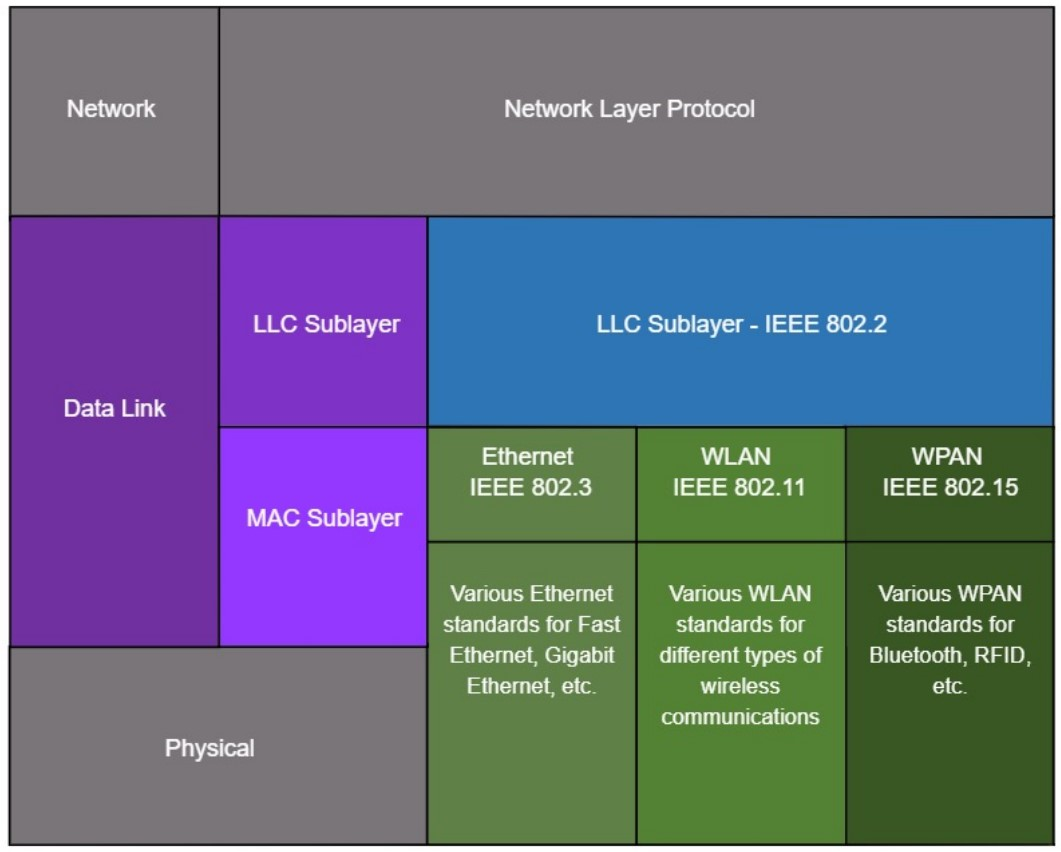
\includegraphics[width=\textwidth]{images/DLL_Sublayers.jpg}
    \caption{Subschichten der Sicherungsschicht / des Data Link Layers (\textsuperscript{\textcopyright}Cisco)}
    \end{center}
\end{figure}

\subsection*{Welches sind die am häufigsten verwendeten Zugriffsverfahren?}
//TODO

\subsection*{Was für Felder findet man in der Sicherungsschicht Frame?}
\begin{itemize}
    \item Head
    \item Data
    \item Trailer
\end{itemize}
//TODO Frame Fields picture, Folie S. 16, Tabelle?

\subsection*{Was sind die wichtigsten Merkmale von MAC Adressen?}\index{MAC-Adresse}
\begin{itemize}
    \item 48 bits = 12 hex-Ziffern = 6 bytes
    \item einzigartig
    \item Erste Hälfte von Hersteller, zweite Hälfte zufällig
\end{itemize}
Beispiel Darstellung einer MAC-Adresse: 3D-8F-45-27-3C-1A oder 3D:8F:45:27:3C:1A

\subsection*{Was machen Endgeräte, wenn ihre NIC ein Frame im Medium erkennen?}
//TODO: Glossareintrag NIC: Network Interface Controller/Card, Netzwerkkarte.\\


\subsection*{Wie werden Sicherungsschicht Frames in einem Switch bearbeitet? }
//TODO Folie S. 21 ff

\subsection*{Wie funktioniert der «Learn-and-forward» Prozess?}
//TODO Folie S. 24 ff

\subsection*{Was ist der Unterschied zwischen «Unicast» und «Broadcast» Frames?}
//TODO

\subsection*{Was ist der Zweck ARPs?}
Das Address Resolution Protocol vermittelt zwischen der Sicherungsschicht - Data Link (2) und der Vermittlungsschicht - Network (3). Es dient dazu, zu einer Netzwerkadresse der Internetschicht (IPv4-Adresse) die physische Adresse der Sicherungsschicht (MAC-Adresse) zu ermitteln. Die ermittelte MAC-Adresse wird in einer ARP-Tabelle hinterlegt.

\subsection*{Wie funktioniert ARP?}
//TODO